\chapter{Introducción}

Este Trabajo de Fin de Grado consiste en construir una solución software
capaz de registrar, exportar y visualizar información sobre la recolección de cultivos
leñosos haciendo uso de un sistema de control embebido.

Este proyecto es software libre, y está liberado con
la licencia \textbf{GNU Affero General Public License} \cite{agplv3}.

\section{Motivación}

En España existen 23.848.757 hectáreas de superficie agrícola utilizada%
\footnote{%
Según el INE, conjunto de la superficie de tierras labradas y tierras
para pastos permanentes.
}%
al aire libre, de las cuales \textbf{4.657.182 hectáreas se dedican a cultivos leñosos}
 \cite{INEdistribucionDeLaSuperficiePorTamaño}.
Entre estos predominan el cultivo del olivar, del viñedo, de los cítricos,
de los frutos secos como las almendras o los pistachos y otros frutales
 \cite{INEpanoramicaCensoAgrario}.

\begin{figure}[!b]
    \centering
    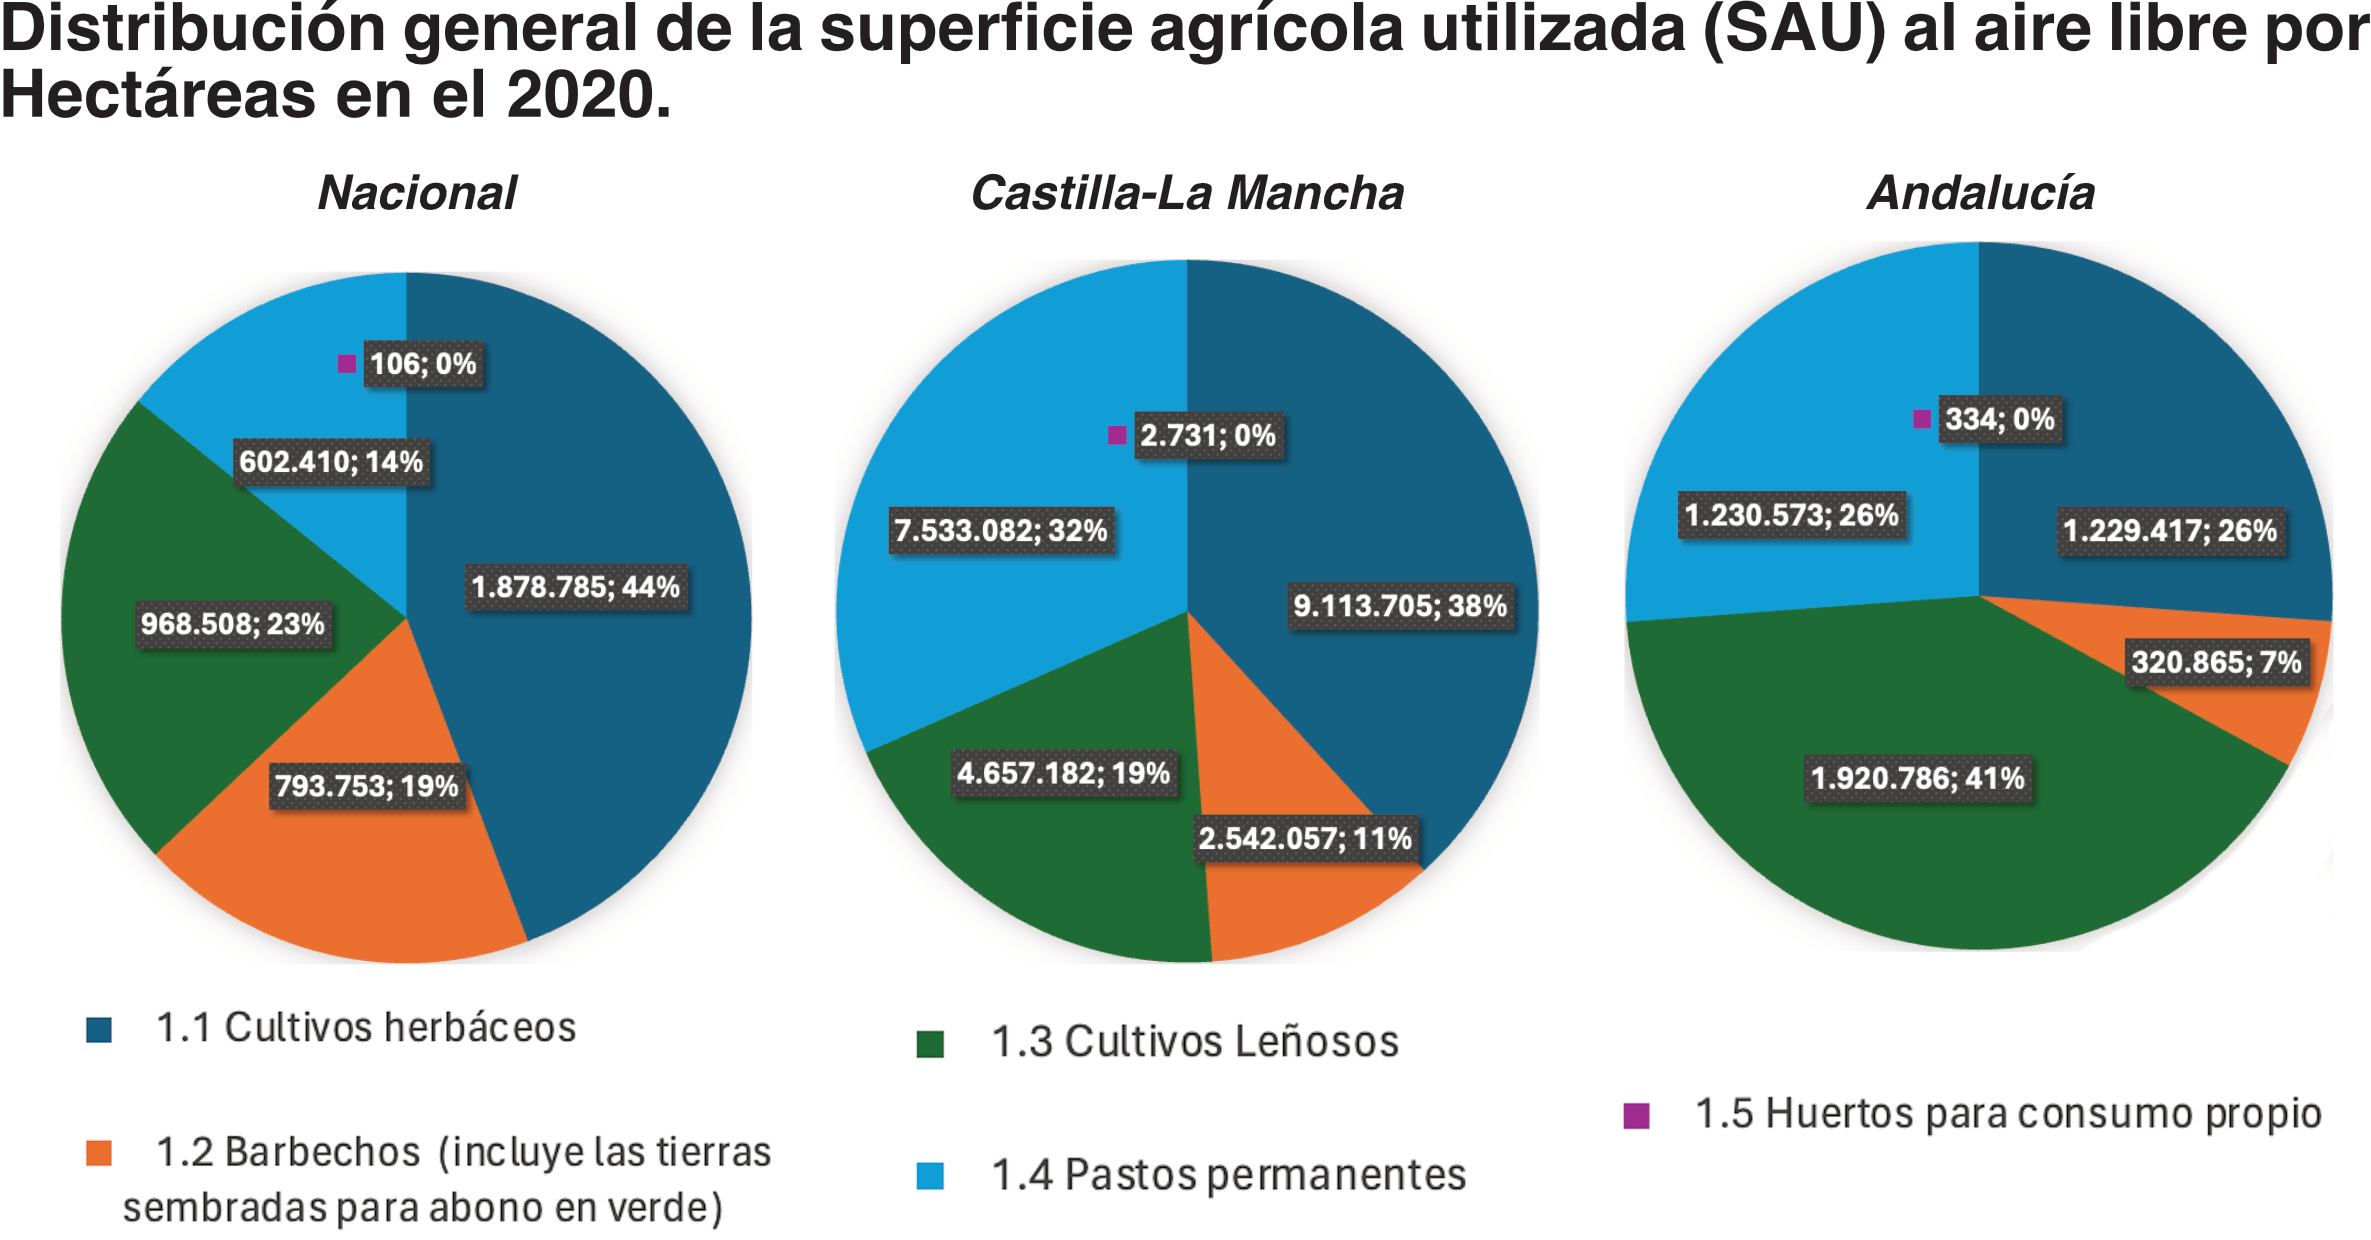
\includegraphics[width=\textwidth]{distribucion-SAU-segun-cultivo-aire-libre.png}
    \caption{\textit{Distribución general de la SAU al aire libre por hectáreas
    según \cite{INEdistribucionDeLaSuperficiePorTamaño}. Los territorios de Andalucía y Castilla-La Mancha
    acumulan aproximadamente el 62\% de los cultivos leñosos en territorio nacional.
    Elaboración propia.}}
\end{figure}

\subsection{Situación de las explotaciones agrícolas en España}

\textbf{La explotación} de la superficie agrícola utilizada \textbf{se realiza mayoritariamente por personas
físicas}. \textbf{Observamos un mayor número de sociedades mercantiles
a medida que aumenta el tamaño de explotación}, siendo el 30\% de quienes explotan los latifundios\footnote{%
    Consideramos que una explotación agrícola es un latifundio a partir de las 100 hectáreas.
}%
 en España
 \cite[Personalidad jurídica según el tamaño de explotación]{INEpanoramicaCensoAgrario}.

\textbf{No existe apenas una renovación de los jefes de explotación}%
\footnote{%
    Según Eustat, la persona física responsable de las actividades financieras y de producción, corrientes y cotidianas de una explotación agrícola.
}%
, con un porcentaje de gestores menores de 45 años
inferior al 40\% en todas las comarcas. La formación reglada específica de los jefes en el caso de
las explotaciones agrarias es inferior al 25\% en todas las comarcas españolas,
llegando a menos del 2,84\% regiones en las que predominan los cultivos leñosos
 \cite[Formación de los jefes de explotación]{INEpanoramicaCensoAgrario}.

La rentabilidad de las explotaciones agrarias ha disminuido en los últimos años. La superficie agrícola
utilizada ha disminuido aproximadamente un 7\% desde el censo agrario del INE del 2009
 \cite[Tamaño y número de las explotaciones agrícolas]{INEpanoramicaCensoAgrario}.

\subsection{Gestión de las explotaciones de cultivos leñosos}

\begin{figure}[!b]
    \centering
    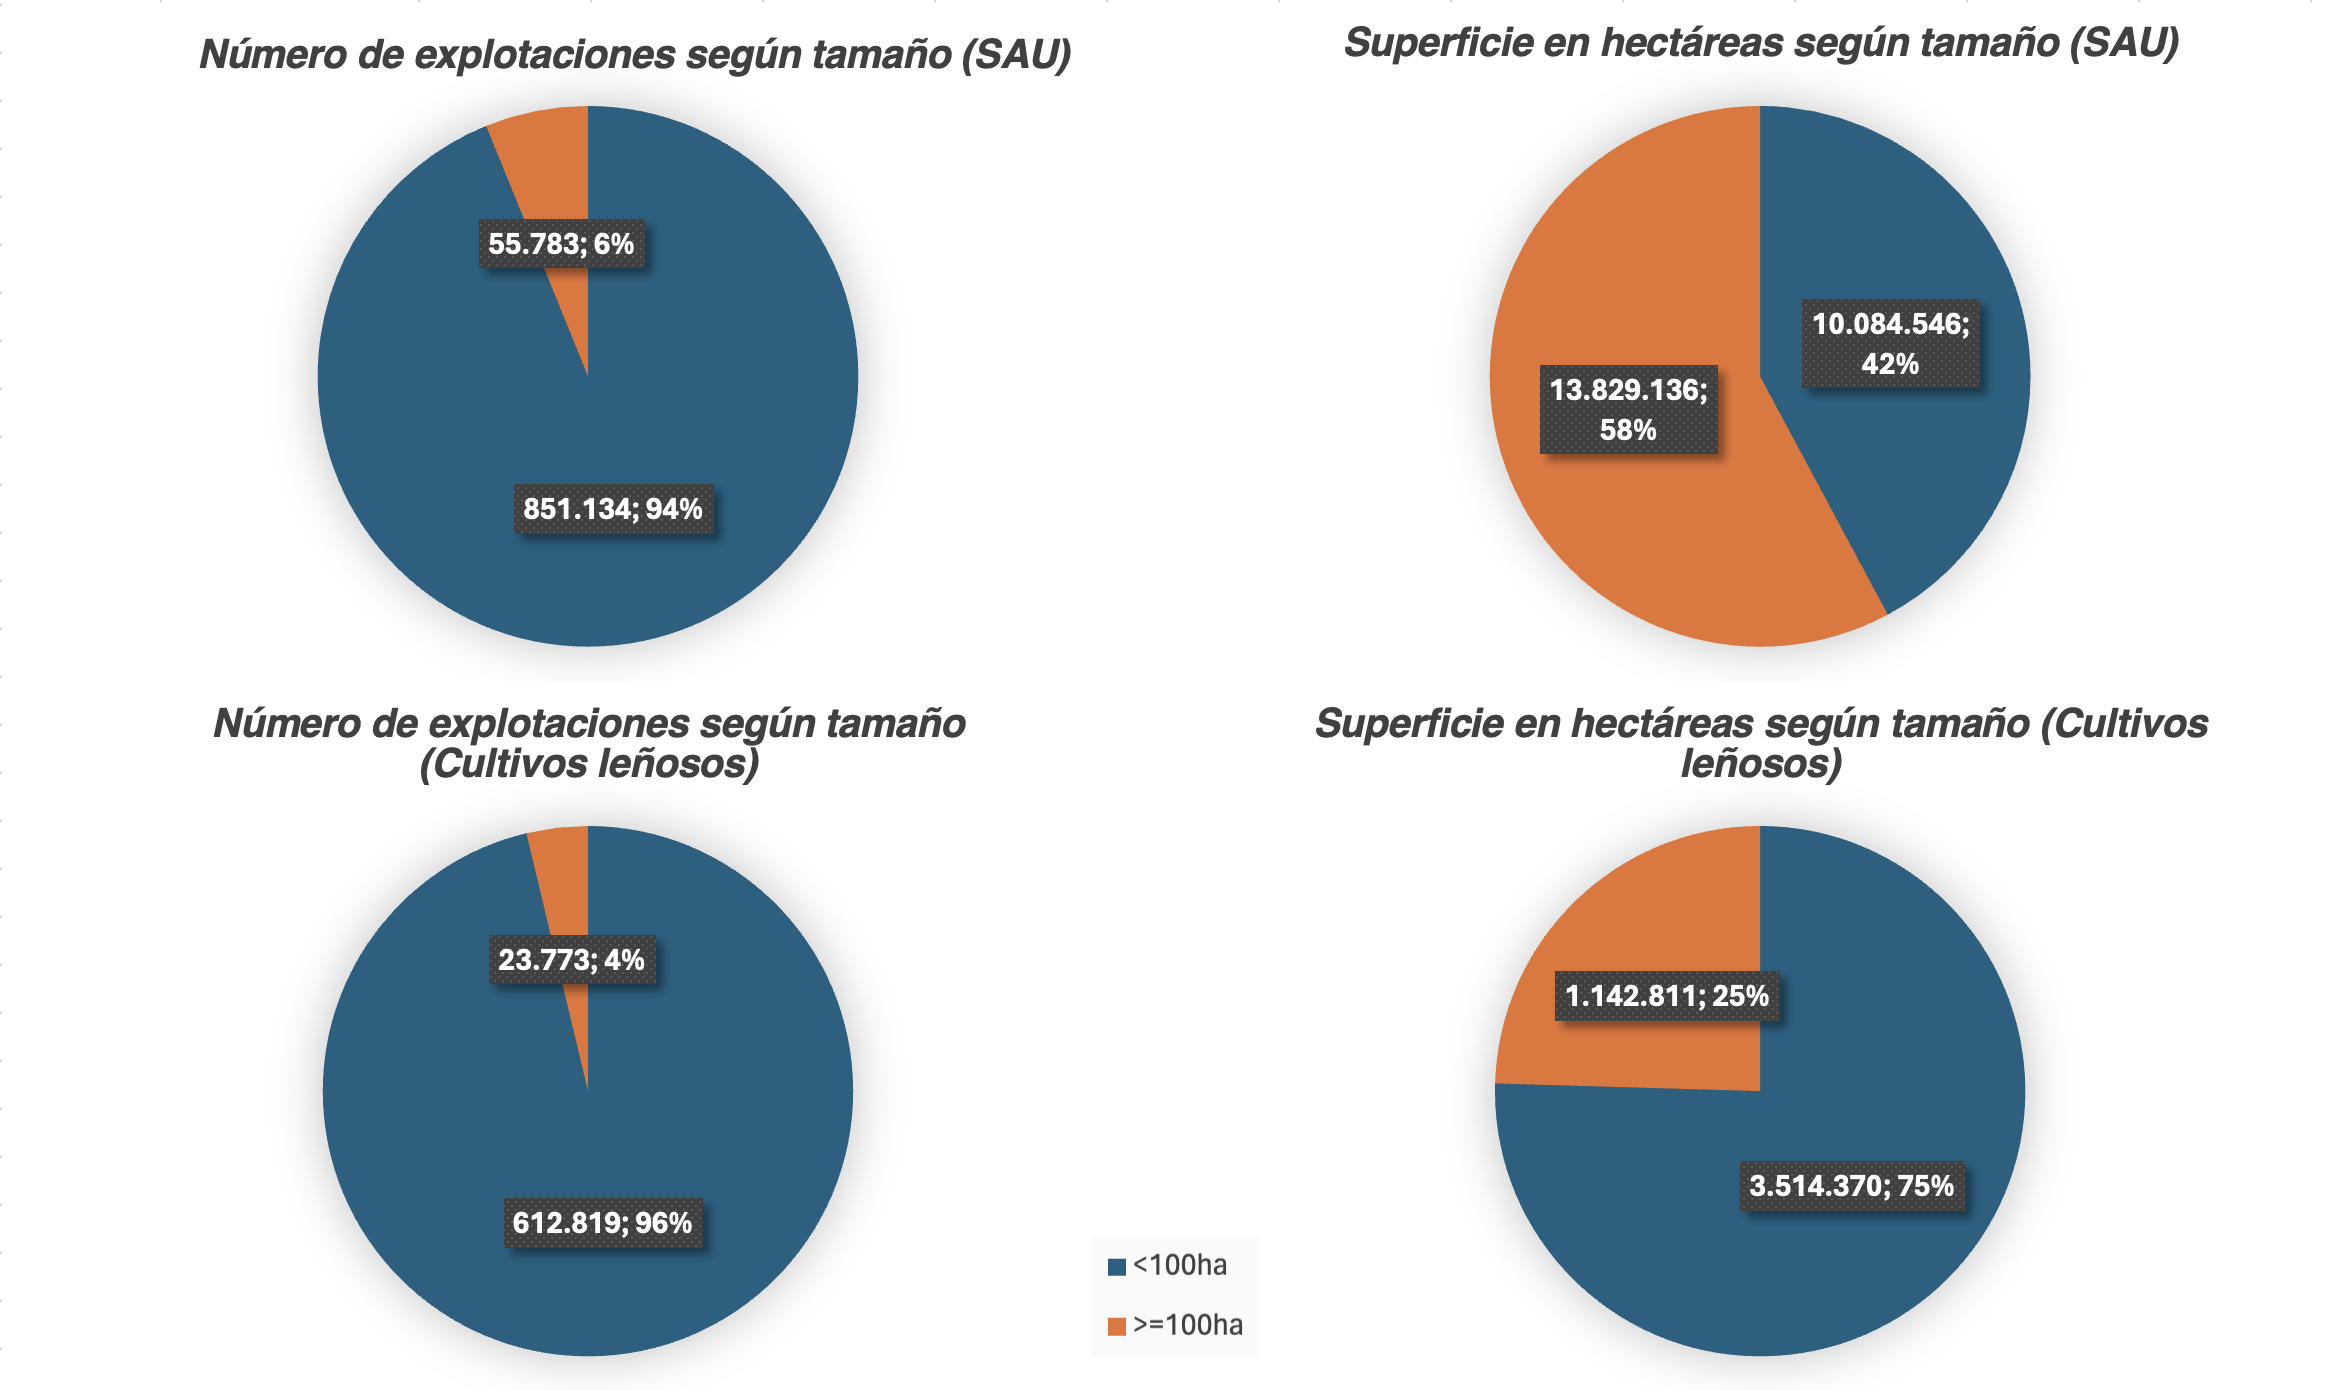
\includegraphics[width=\textwidth]{distribucion-SAU-segun-tamaño.png}
    \caption{\textit{Distribución general de la SAU por tamaño de la explotación según
    \cite{INEdistribucionDeLaSuperficiePorTamaño}. Apreciamos que, aunque es similar la
    proporción del número de explotaciones según el tamaño para la media de todos los tipos
    de cultivos y para los leñosos, la superficie ocupada para ambas categorías difiere
    significativamente. Elaboración propia.}}
\end{figure}

Encontramos la mayor superficie de cultivos leñosos en la mitad sur de la península,
destacando Andalucía, Castilla-La Mancha y Extremadura.
\cite[Reparto de la superficie dedicada a los grandes cultivos.]{INEpanoramicaCensoAgrario}

\textbf{Dos terceras partes del coste} de este tipo de cultivos \textbf{se destinan a la
recolección y a la poda}
 \cite{Mecaolivar}.
Entre las soluciones mecanizadas para la recolección encontramos principalmente
los vareadores eléctricos y los paraguas vibradores,
mientras que para la poda las tijeras eléctricas, las motosierras y
las trituradoras para motocultores.

El \textbf{encarecimiento de la mano de obra}, la \textbf{importación de producto de países con menor coste de
producción} y el \textbf{bajo nivel de automatización y de inversión} por parte
de los propietarios de las explotaciones agrarias probablemente sean 
algunas de las causas que hayan hecho que la rentabilidad de la que
hablábamos en el anterior apartado haya disminuido en los últimos años.

\subsection{Externalización de la recolecta de cultivos leñosos a empresas especializadas}

\textbf{Algunos jefes de explotación deciden externalizar la recolección
de sus cultivos a empresas especializadas}. Ocurre un problema en este
caso, y es que el jefe de explotación deja de tener la certeza de que la
recolección se ha realizado de forma correcta, y de que la cantidad de producto
recolectado es la que se espera. Este problema también se da en otros contextos,
como el de grandes fincas profesionalizadas.

\textbf{Nuestro cliente acude a nosotros para desarrollar una solución propia de
estadísticas de recolección en cultivos leñosos.}

\section{Objetivo}

Con este proyecto \textbf{queremos obtener un producto que genere informes
de trabajo de un paraguas vibrador}, de forma que permita tanto a
quien recolecta el fruto como al jefe de explotación tener información
acerca de una jornada de trabajo para certificar el trabajo realizado.

Concretamente, según veremos en el capítulo dedicado al análisis del problema,
buscamos \textbf{desarrollar
una solución software que permita registrar, exportar y visualizar
información sobre la recolección de cultivos
leñosos con paraguas vibradores según los criterios de nuestro cliente},
con la restricción de que el registro y el exportado pueda ejecutarse en
una plataforma hardware ya distribuida en el mercado.

\section{Estructura del documento}

Esta memoria refleja el proceso de desarrollo de la solución software.
Cada una de las secciones expuestas representa una etapa del desarrollo.
\textbf{Etapas posteriores se basan en las anteriores, y pueden corregirlas.}
Si se corrigen, lo indicamos.

\begin{enumerate}
    \item \textbf{Introducción.} Donde exponemos el problema a resolver de forma general,
    sus circunstancias actuales y los objetivos que se quieren alcanzar en rasgos generales.

    \item \textbf{Planificación.} Donde exponemos cómo abordamos el desarrollo del problema.
    Explicamos qué metodología seguimos, cómo estimamos el tiempo y los costes, cómo seguimos el progreso
    del proyecto y cómo registramos métricas para los objetivos del sexto capítulo de esta memoria.

    \item \textbf{Problema a resolver.} Donde describimos el problema de una forma clara y concisa.
    Enunciamos qué se quiere resolver, quién va a interactuar con el programa y en qué circunstancias
    se interactuaría con el programa.

    \item \textbf{Arquitectura del sistema.} Donde enumeramos distintas soluciones arquitectónicas
    plausibles y elegimos una de ellas junto al cliente.

    \item \textbf{Implementación.} Donde describimos cómo llevamos a cabo el desarrollo software
    de la solución propuesta.
    \begin{itemize}
        \item Escucha y registro de eventos.
        \item Almacenamiento en memoria persistente.
        \item Extracción de datos.
        \item Firma de los datos.
        \item Transmisión de los datos.
        \item Visualización de los datos.
    \end{itemize}

    \item \textbf{Comparación de los datos previos, durante y posteriores al desarrollo.} Donde evaluamos cómo de
    acertados fueron los análisis del segundo, tercer y cuarto capítulo de esta memoria.

    \item \textbf{Conclusión.} Donde realizamos una visita crítica a las ideas de los puntos
    anteriores una vez finalizado el proyecto y exponemos nuevas ideas surgidas de la experiencia.
\end{enumerate}
